\documentclass[a4j,10pt]{jsarticle}
\usepackage{layout,url,resume}
\usepackage[dvipdfmx]{graphicx}
\pagestyle{empty}

\begin{document}
%\layout

\title{スマートフォンのブラウザで視聴中のWebページ・動画の視聴位置を保存・復旧するしおりアプリ}

% 和文著者名
\author{
    Arch B3 新真虎(masatora) \thanks{慶應義塾大学環境情報学部}
    \and
    Adviser: 松谷健史(macchan) \thanks{慶應義塾大学大学院 政策・メディアメディア研究科特任講師}
}

\maketitle
\thispagestyle{empty}

\section{背景}
スマートフォンでネットサーフィンをしているとき、
読んでいる途中のページや動画を保存したいというニーズがある。
そうしたニーズに対応するブックマークアプリはすでに存在する\cite{Pocket}\cite{instapaper}。

しかし、既存のブックマークアプリには以下の問題がある。
\begin{enumerate}
\item 保存したWebページのスクロール位置がわからなくなる
\item 保存した動画の再生位置(何分何秒まで見ていた・何分何秒が面白かった)がわからなくなる
\end{enumerate}

その結果、Webページや動画の視聴を再開したり、誰かに共有するたびに、
どこまで読んでいたか・見ていたかを探す時間が無駄になってしまう。

%---------------------------------------------

\section{目的}
上記の問題を解決するため、スマートフォンで見ているWebページや動画をどこまで読んでいたか・
どこまで見ていたかという情報とともに保存し、復旧できるようにすることを目指す。

\section{アプローチ}
Webページおよび動画のスクロール位置や再生位置を保存・復旧することのできる
iOSアプリケーションを開発する\cite{shiori-web-for-safari}。

\section{環境}
\begin{itemize}
\item Xcode12
\item Swift5
\item ECMAScript 2015
\end{itemize}

\section{実装}
\subsection{ユーザーフロー}
ユーザーがこのアプリケーションを使用してWebページ・動画を保存し、
復旧するまでの主な手順を以下に示した。
\begin{enumerate}
\item SafariでWebページや動画を視聴している
\item 共有ボタンをタップ
\item 「Shiori」ボタンをタップして保存する
\item アプリを開くと、視聴していたWebページ・動画が保存されている
\item 保存したWebページ・動画をタップすると、スクロール位置・再生位置が復旧された状態でWebページ・動画が開かれる
\end{enumerate}

\subsection{実装詳細}
上記の機能を実現するため、Appleが提供するApp Extension\cite{App-Extension}の
一種であるShare Extension\cite{Share-Extension}という機能を利用する。
Share Extensionとは、iPhoneで開いているWebページや動画を
任意のアプリケーションに保存できる機能である。
Share Extensionを利用してアプリにWebページや動画を保存するタイミングで
Javascriptコードを実行し、以下の二つのデータを取得する。
\begin{itemize}
\item スクロール位置
\item 動画の再生時間
\end{itemize}

そして、取得したデータをWebページや動画のメタデータとして保存する。
ユーザーが保存したWebページや動画をクリックすると、アプリケーション内部で
ブラウザを開き、スクロール位置や再生位置を復旧させた状態でWebページや動画を開く。


\section{評価}
評価のために、開発したアプリケーションが以下の2つの機能を実現できていることを確認する。
\begin{enumerate}
\item 保存したWebページのスクロール位置が復旧できること
\item 保存した動画の再生位置が復旧できること
\end{enumerate}

評価の方法として、実際に任意のWebページ・動画を途中までスクロール・再生した上で
アプリケーションに保存する。保存されたWebページ・動画をアプリケーション内で開き、
保存したときのスクロール位置・再生位置が復旧するかどうか検証する。

検証には、以下のWebページ・動画を使用した。
\begin{enumerate}
\item Webページ: ネットの父・村井純が見る未来#01/理想だけを追えばいい時代が来る\cite{murai-web-page}
\item 動画: 「インターネット文明」村井純\cite{murai-video}
\end{enumerate}

\section{結果}
\subsection{実現できたこと}
\subsubsection{保存したWebページのスクロール位置を復旧}
評価の結果、図\ref{fig:one}, 図\ref{fig:two}のように、保存したWebページのスクロール位置が復旧することを確認できた。
\begin{figure}[htbp]
    \begin{minipage}{0.5\hsize}
        \begin{center}
        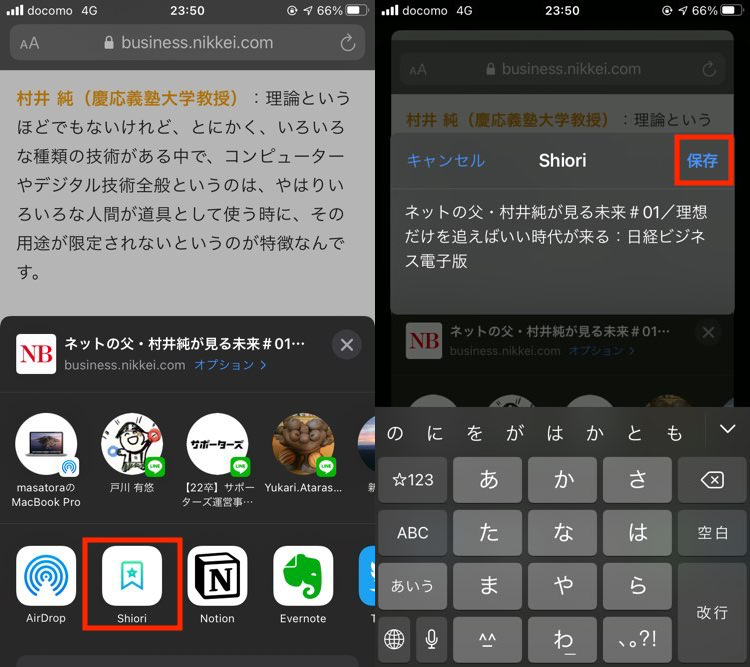
\includegraphics[width=70mm]{../assets/scroll_position/scroll_position1.png}
        \end{center}
        \caption{}
        \label{fig:one}
    \end{minipage}
    \begin{minipage}{0.5\hsize}
        \begin{center}
        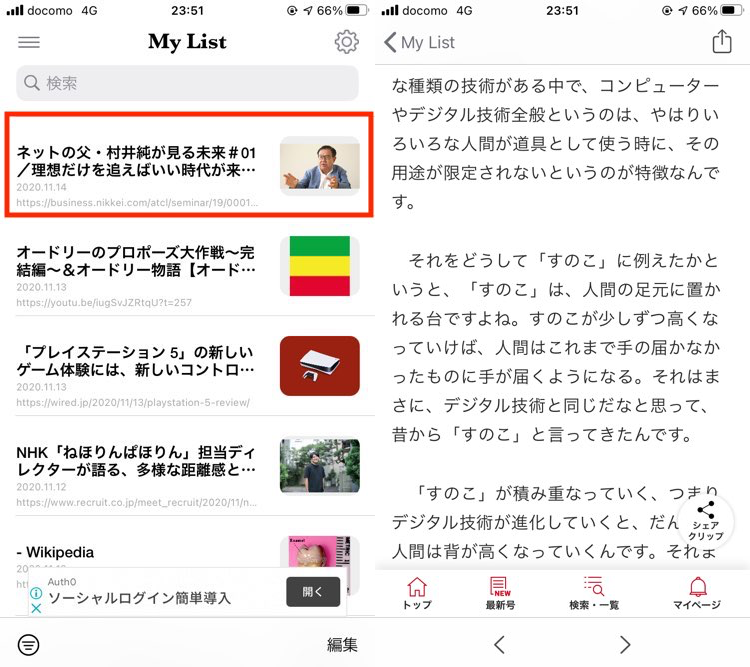
\includegraphics[width=70mm]{../assets/scroll_position/scroll_position2.png}
        \end{center}
        \caption{}
        \label{fig:two}
    \end{minipage}
\end{figure}

\subsubsection{保存した動画の再生位置が復旧できることを確認}
評価の結果、図\ref{fig:three}, 図\ref{fig:four}のように、保存した動画の再生位置が復旧することを確認できた。
\begin{figure}[htbp]
    \begin{minipage}{0.5\hsize}
        \begin{center}
        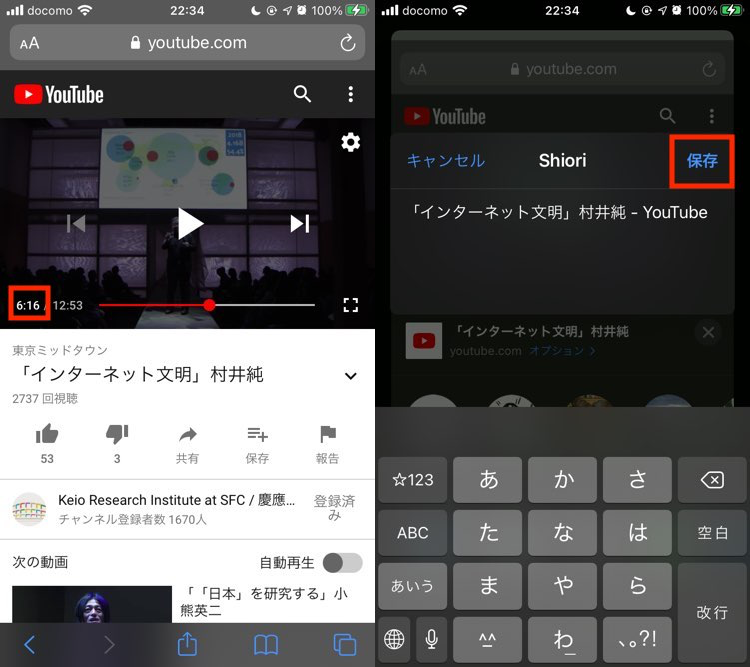
\includegraphics[width=70mm]{../assets/playback_position/playback_position1.png}
        \end{center}
        \caption{}
        \label{fig:three}
    \end{minipage}
    \begin{minipage}{0.5\hsize}
        \begin{center}
        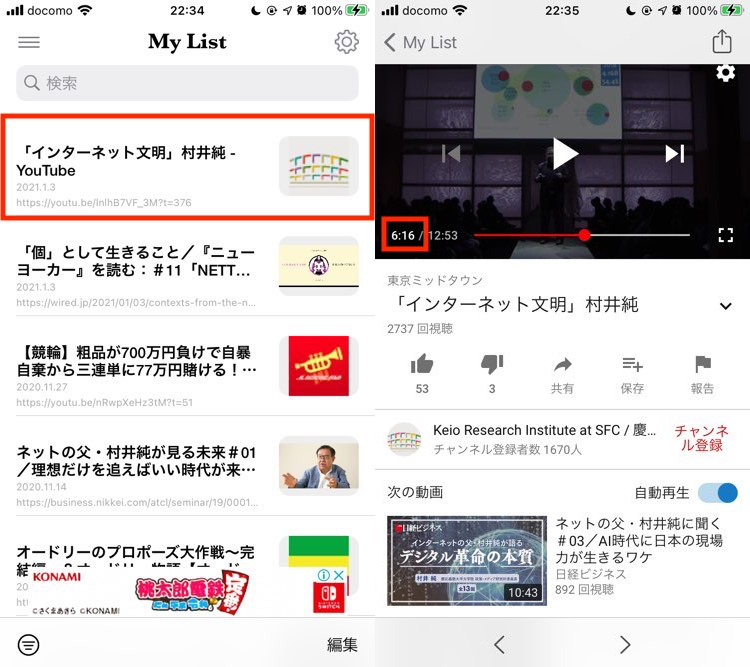
\includegraphics[width=70mm]{../assets/playback_position/playback_position2.png}
        \end{center}
        \caption{}
        \label{fig:four}
    \end{minipage}
\end{figure}

\subsection{実現できていないこと}
一方、実現できていない点は以下である。
\begin{itemize}
\item 一部対応できていない動画サイトが存在する
\end{itemize}

\bibliographystyle{junsrt}
\bibliography{resume}

\end{document}
% end of file
